\begin{normalsize}

\subsection{VDW(3, 3)}

Известно, что $W(3, 3) = 27$.

Но мы снова докажем худшую оценку.

Обозначим наши цвета $R, B, G$ и рассмотрим произвольную раскраску $\chi: \{1, \ldots, W\} \to \{R, B, G\}$.

Рассмотрим разбиение $\{1, \ldots, W\}$ на блоки длины $7$ --- можем считать, что $W$ делится на $7$.

\[ \{1, 2, \ldots, 7\}, \{8, \ldots, 14\}, \ldots, \{W-6, \ldots, W\}. \]

Внутри блока $B_i$ длины $7$ есть арифметическая прогрессия, в которой первые два элемента окрашены одинаково.

Аналогично предыдущему случаю, получаем что существует $U$ и $a, d, D$, такие что:

\begin{itemize}
    \item $\chi(a) = \chi(a + d) = \chi(a + D) = \chi(a + D + d) = R$.
    
    \item $\chi(a + 2d) = \chi(a + D + 2d) = B$.
    
    \item $a + 2D + 2d \leq U$.
\end{itemize}

\begin{center}
    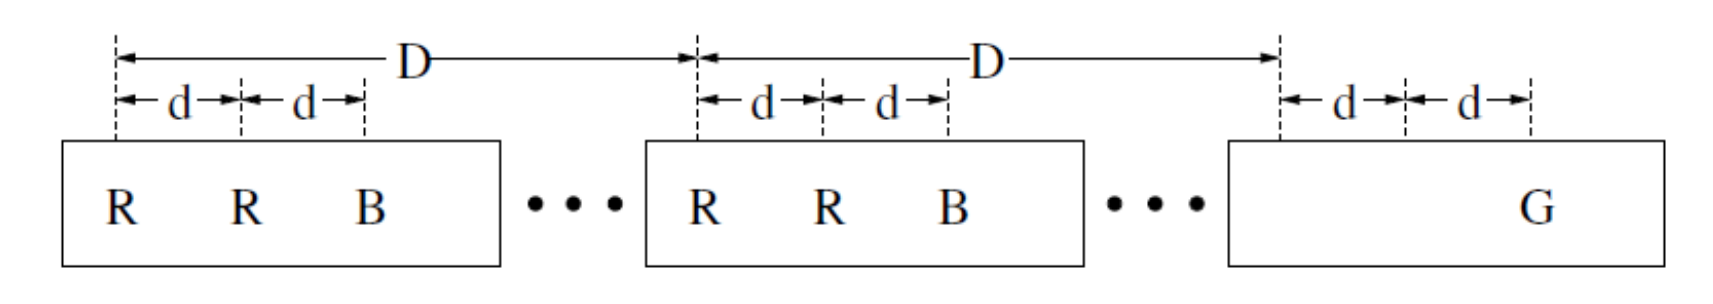
\includegraphics[width=0.7\textwidth]{par49vdw33.png}
\end{center}

Если $\chi(a + 2D + 2d) = B$, то 

\[ \chi(a + 2d) = \chi(a + D + 2d) = \chi(a + 2D + 2d) = B. \]

Если $\chi(a + 2D + 2d) = R$, то

\[ \chi(a) = \chi(a + D + d) = \chi(a + 2D + 2d) = R. \]

В этом случае получаем $\chi(a + 2D + 2d) = G$.

Доказали лемму:

\begin{lemma}
    Существует $U$, такое что с точностью до переобозначения цветов, для всех $3$-раскрасок $\{1, \ldots, U\}$ выполняется одно из следующих условий:

    \begin{enumerate}
        \item Существует одноцветная $3$-а.п.
        
        \item Существует две $3$-а.п., такие что:
        
        \begin{itemize}
            \item Одна окрашена RRG,
            
            \item Одна окрашена BBG,
            
            \item У них общая третья точка.
        \end{itemize}
    \end{enumerate}
\end{lemma}

Рассмотрим разбиение $\{ 1, \ldots, W \}$ на блоки длины $U$.

Ключевая идея: рассмотреть разбиение на блоки, которые в свою очередь разбиты на более мелкие блоки.

Рассмотрим $3^{|U|}$-раскраску $\{1, \ldots, W\}$, и возьмем $W$ достаточно большим, чтобы существовало два одинаково раскрашенных блока $B_i$ и $B_j$ и третий блок $B_k$, формирующий с ними а.п. из блоков.

\begin{center}
    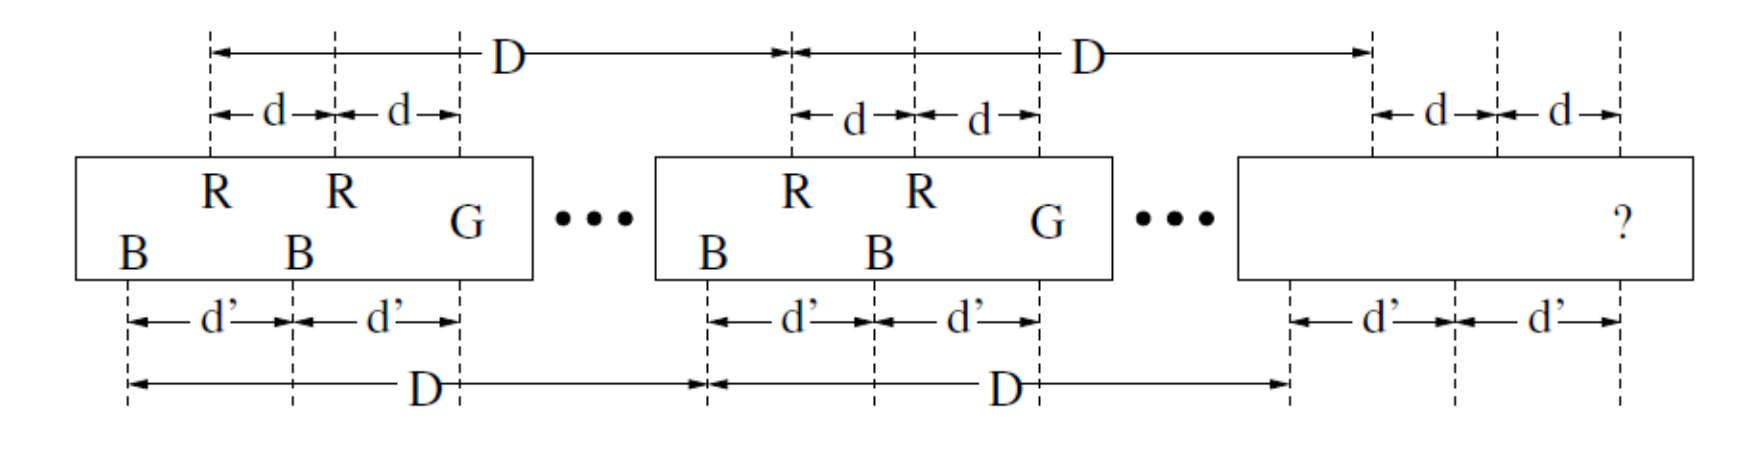
\includegraphics[width=0.7\textwidth]{par49vdw33-2.png}
\end{center}

Какой бы цвет мы не выбрали, найдется а.п.

\end{normalsize}

\begin{exerc}
    Константы и формулировка VDW(3, 3)
\end{exerc}

\begin{notice}
    Аналогично можно доказать VDW(3, c)
\end{notice}